%==============================================================================
%  MATH 231 -- Linear Algebra I (Queens College, Fall 2026)
%  MATRIX UNIT, PART 10 -- Cramer's Rule, the Inverse, and the
%  Pseudo-inverse
%
%  Section numbering runs CONTINUOUSLY across the parts of the matrix unit;
%  see Part 2's header for the full map.  This part is Sections 50-54, hence
%  \setcounter{section}{49}.
%
%  STATUS: complete.  Sections 50-54.  Written from the plan in
%  plan/MATH231_remaining_units_plan.tex (2026-10-25).
%
%  AUDIENCE: distributed to students.  No instructor-facing apparatus.
%
%  WHAT THE INSTRUCTOR SPECIFIED, AND WHERE IT IS.
%   - Cramer's rule with geometric intuition: Sec. 50 (the 2x2 area picture
%     in Sec. 50.3).
%   - Generalization of the inverse: Sec. 51.  Computing the inverse by the
%     adjoint: Sec. 52.  General properties of the inverse (det etc.):
%     Sec. 53.
%   - After the inverse is generalized, the (Moore-Penrose) pseudo-inverse:
%     Sec. 54.
%
%  DECISIONS CARRIED FROM THE PLAN.
%
%   D3. Sec. 51.3 proves that a one-sided inverse of a square matrix is
%       two-sided (via rank-nullity), and draws the consequence promised in
%       Sec. 20.6: Q'Q = I alone forces QQ' = I, and Q^{-1} = Q'.
%
%   D7. The least-squares formula x = (A'A)^{-1} A'b first appears in
%       Sec. 53.4, now that the inverse exists.
%
%   D8. PSEUDO-INVERSE SCOPE: full column rank, full row rank, invertible,
%       the four Moore-Penrose conditions, and one rank-one (rank-deficient)
%       example checked against them.  Existence and uniqueness for every A
%       is STATED; the general construction is via the SVD, at the end of the
%       course.
%
%   N4. "ADJOINT".  The instructor's list says "computing the inverse by the
%       adjoint".  The document says ADJUGATE, adj(A), and explains once that
%       "classical adjoint" is the older name for the same matrix, while
%       "adjoint" elsewhere usually means the (conjugate) transpose.
%
%  DATA.  Sec. 53.4 and Sec. 54.2 reuse the line fit of Sec. 49.4 (points
%  (1,1), (2,2), (3,2); answer [2/3, 1/2]).
%
%  Compile with pdflatex or tectonic (standard TeX Live packages only; uses
%  tikz).
%==============================================================================
\documentclass[11pt]{article}

\usepackage[margin=1in]{geometry}
\usepackage{amsmath,amssymb,amsthm}
\usepackage[dvipsnames]{xcolor}
\usepackage{enumitem}
\usepackage{booktabs}
\usepackage{array}
\usepackage[hidelinks]{hyperref}
\usepackage{titlesec}
\usepackage{needspace}
\usepackage{tikz}
\usetikzlibrary{arrows.meta}

%------------------------------------------------------------------ style ----
\titleformat{\section}{\large\bfseries\sffamily}{\thesection.}{0.6em}{}
\titleformat{\subsection}{\normalsize\bfseries\sffamily}{\thesubsection.}{0.5em}{}
\titlespacing*{\section}{0pt}{14pt}{6pt}
\setlength{\emergencystretch}{3em}

\theoremstyle{plain}
\newtheorem{thm}{Theorem}[section]
\newtheorem{lem}[thm]{Lemma}
\newtheorem{cor}[thm]{Corollary}

\theoremstyle{definition}
\newtheorem{defn}{Definition}[section]
\newtheorem{ex}{Example}[section]
\theoremstyle{remark}
\newtheorem*{rmk}{Remark}
\newtheorem*{warn}{A common confusion}

\newcommand{\lookahead}{\par\smallskip\noindent
  \textbf{\sffamily\textcolor{RoyalBlue}{Looking ahead.}}\ \ignorespaces}
\newcommand{\lookback}[1][the vector unit]{\par\smallskip\noindent
  \textbf{\sffamily\textcolor{ForestGreen}{From #1.}}\ \ignorespaces}

%--------------------------------------------------------------- notation ----
\newcommand{\R}{\mathbb{R}}
\newcommand{\vc}[1]{\mathbf{#1}}
\newcommand{\mt}[1]{\mathbf{#1}}
\newcommand{\norm}[1]{\lVert #1\rVert}
\newcommand{\T}{^{\mathsf{T}}}
\newcommand{\colsp}[1]{\operatorname{col}[#1]}
\newcommand{\rowsp}[1]{\operatorname{row}[#1]}
\newcommand{\nullsp}[1]{\operatorname{null}[#1]}
\newcommand{\xh}{\hat{\vc{x}}}
\DeclareMathOperator{\spanop}{span}
\DeclareMathOperator{\diagop}{diag}
\DeclareMathOperator{\rank}{rank}
\DeclareMathOperator{\adj}{adj}
\newenvironment{aug}[1]{\left[\begin{array}{#1}}{\end{array}\right]}

%------------------------------------------------------------- tikz helpers --
\tikzset{
  vecarr/.style   = {-{Stealth[length=2.6mm,width=2.0mm]},very thick},
  thinarr/.style  = {-{Stealth[length=2.2mm,width=1.7mm]},thick},
  axisline/.style = {->,gray!75,thin}
}

\title{\vspace{-1.2cm}\textbf{\sffamily MATH 231 -- Linear Algebra I}\\[4pt]
       {\large\sffamily The Matrix Unit, Part 10 \textbullet\ Cramer's Rule,
        the Inverse, and the Pseudo-inverse}\\[2pt]
       {\normalsize\sffamily Kiely Hall 326 \textbullet\
        Instructor: Kevin Bedoya}}
\author{}
\date{}

\begin{document}
\setcounter{section}{49}  % this part opens at Section 50; see the header note
\maketitle
\vspace{-1.6cm}

\noindent\textbf{About this document.} This is Part 10 of the matrix unit,
Sections 50--54. Section numbers run continuously through the unit (Part 2's
opening table lists them all).

\medskip
\noindent\textbf{Assumed.} The determinant, its laws D1--D10 and cofactors
(Part 7); the $2\times2$ determinant as an area and its column properties
(\S22--\S23); the $2\times2$ inverse (\S34); null space and rank--nullity (Part
6); elimination (Part 8); least squares and the normal equations (Part 9);
orthogonal projections (\S27).

\medskip
\noindent\textbf{What you should be able to do afterwards.} Solve a small system by
Cramer's rule and explain it with areas; state the equivalent conditions for an
$n\times n$ matrix to be invertible; prove that a one-sided inverse of a square
matrix is two-sided; compute an inverse by Gauss--Jordan elimination and by the
adjugate; use the algebraic properties of the inverse; and compute and recognise
the pseudo-inverse of a matrix with full column rank, with full row rank, or of
rank one.

%==============================================================================
\section{Cramer's rule}
%==============================================================================

%------------------------------------------------------------------------------
\subsection{The statement}
%------------------------------------------------------------------------------
\begin{thm}[Cramer's rule]
\label{thm:cramer}
Let $\mt{A}\in\R^{n\times n}$ with $\det\mt{A}\neq0$, and let $\mt{A}_i(\vc{b})$
denote $\mt{A}$ with its $i$-th column replaced by $\vc{b}$. Then the unique
solution of $\mt{A}\vc{x}=\vc{b}$ is given, entry by entry, by
\[
  \boxed{\;x_i=\frac{\det\mt{A}_i(\vc{b})}{\det\mt{A}},\qquad i=1,\dots,n.\;}
\]
\end{thm}

\begin{ex}
The system of Part 1 \S1.5,
$\begin{bmatrix}2&1\\1&3\end{bmatrix}\vc{x}=\begin{bmatrix}5\\5\end{bmatrix}$, has
$\det\mt{A}=5$ and
\[
  x_1=\frac{1}{5}\det\begin{bmatrix}5&1\\5&3\end{bmatrix}=\frac{15-5}{5}=2,
  \qquad
  x_2=\frac{1}{5}\det\begin{bmatrix}2&5\\1&5\end{bmatrix}=\frac{10-5}{5}=1 .
\]
\end{ex}

%------------------------------------------------------------------------------
\subsection{Why it should be true: areas}
%------------------------------------------------------------------------------
In the plane the rule is a statement about parallelograms. The solution says
$\vc{b}=x_1\vc{a}_1+x_2\vc{a}_2$. Compare two parallelograms that share the side
$\vc{a}_2$: the one on $\vc{a}_1,\vc{a}_2$, of area $|\det\mt{A}|$ (\S23), and
the one on $\vc{b},\vc{a}_2$, of area $|\det\mt{A}_1(\vc{b})|$.
\begin{itemize}[leftmargin=1.4em,itemsep=3pt]
  \item Sliding $\vc{b}$ parallel to $\vc{a}_2$, back to $x_1\vc{a}_1$, is a
        shear of the parallelogram on $\vc{b},\vc{a}_2$. It keeps the base
        $\vc{a}_2$ and the height, so it keeps the area (\S18.3, \S22 P7).
  \item The parallelogram on $x_1\vc{a}_1,\vc{a}_2$ is the one on
        $\vc{a}_1,\vc{a}_2$ stretched by $x_1$ in one direction, so its area is
        $|x_1|$ times as large.
\end{itemize}
So $\text{area}(\vc{b},\vc{a}_2)=|x_1|\cdot\text{area}(\vc{a}_1,\vc{a}_2)$, and
with signs, $x_1=\det[\,\vc{b}\ \vc{a}_2\,]/\det[\,\vc{a}_1\ \vc{a}_2\,]$. The
unknown $x_1$ is a ratio of areas.

\begin{center}
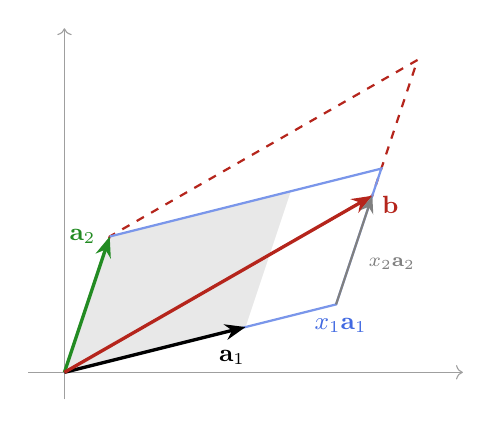
\begin{tikzpicture}[scale=1.15]
  \draw[axisline] (-0.4,0) -- (4.4,0);
  \draw[axisline] (0,-0.3) -- (0,3.8);
  \fill[gray!18] (0,0) -- (2,0.5) -- (2.5,2) -- (0.5,1.5) -- cycle;
  \draw[BrickRed,thick,dashed] (0,0) -- (3.4,1.95) -- (3.9,3.45) -- (0.5,1.5) -- cycle;
  \draw[RoyalBlue!70,thick] (0,0) -- (3,0.75) -- (3.5,2.25) -- (0.5,1.5);
  \draw[vecarr,black] (0,0) -- (2,0.5);
  \draw[vecarr,ForestGreen] (0,0) -- (0.5,1.5);
  \draw[vecarr,BrickRed] (0,0) -- (3.4,1.95);
  \draw[thinarr,gray] (3,0.75) -- (3.4,1.95);
  \node[below right,font=\small] at (1.6,0.35) {$\vc{a}_1$};
  \node[left,font=\small,ForestGreen] at (0.45,1.5) {$\vc{a}_2$};
  \node[right,font=\small,BrickRed] at (3.4,1.85) {$\vc{b}$};
  \node[below,font=\small,RoyalBlue] at (3.05,0.7) {$x_1\vc{a}_1$};
  \node[right,font=\scriptsize,gray] at (3.25,1.2) {$x_2\vc{a}_2$};
\end{tikzpicture}
\end{center}

\noindent The grey parallelogram is spanned by $\vc{a}_1,\vc{a}_2$; the blue by
$x_1\vc{a}_1,\vc{a}_2$; the dashed red by $\vc{b},\vc{a}_2$. Blue and red have
the same base and height, and blue is $x_1$ grey parallelograms long.

%------------------------------------------------------------------------------
\subsection{The proof}
%------------------------------------------------------------------------------
The picture translates into the column laws of the determinant (D6 and D7 of
\S38, in their column form).

\begin{proof}[Proof of Theorem~\ref{thm:cramer}]
Write $\vc{b}=\mt{A}\vc{x}=\sum_{j}x_j\vc{a}_j$ and put it in column $i$:
\[
  \det\mt{A}_i(\vc{b})
  =\det[\,\vc{a}_1\ \cdots\ \textstyle\sum_jx_j\vc{a}_j\ \cdots\ \vc{a}_n\,]
  =\sum_{j}x_j\det[\,\vc{a}_1\ \cdots\ \vc{a}_j\ \cdots\ \vc{a}_n\,],
\]
by linearity in column $i$, where $\vc{a}_j$ now sits in position $i$. For
$j\neq i$ that matrix has $\vc{a}_j$ in two columns, so its determinant is $0$.
Only $j=i$ survives: $\det\mt{A}_i(\vc{b})=x_i\det\mt{A}$.
\end{proof}

\noindent In $\R^{3}$ the same argument reads: $x_i$ is a ratio of volumes.

%------------------------------------------------------------------------------
\subsection{A formula, not an algorithm}
%------------------------------------------------------------------------------
\begin{ex}
Part 1 \S1.6's system, with $\det\mt{A}=3$ (\S42.6):
\[
  \begin{aligned}
  x_1&=\tfrac13\det\begin{bmatrix}5&2&0\\5&1&1\\4&0&1\end{bmatrix}=\tfrac13(5-2)=1,\\
  x_2&=\tfrac13\det\begin{bmatrix}1&5&0\\0&5&1\\1&4&1\end{bmatrix}=\tfrac13(1+5)=2,\\
  x_3&=\tfrac13\det\begin{bmatrix}1&2&5\\0&1&5\\1&0&4\end{bmatrix}=\tfrac13(4+10-5)=3 .
  \end{aligned}
\]
\end{ex}

\noindent Four $3\times3$ determinants, where one elimination did the whole job in
\S42.2. In general Cramer's rule needs $n+1$ determinants of size $n$. That is
hopeless by cofactors and still $n+1$ times the cost of elimination done
sensibly. Its value is that it gives each unknown as an explicit formula in the
entries. That makes it the right tool for proofs, and it produces the inverse
formula of \S52.

%==============================================================================
\section{The inverse of an \texorpdfstring{$n\times n$}{n x n} matrix}
%==============================================================================

%------------------------------------------------------------------------------
\subsection{The definition}
%------------------------------------------------------------------------------
\begin{defn}[Inverse]
$\mt{A}\in\R^{n\times n}$ is \textbf{invertible} (or \textbf{nonsingular}) if
there is a matrix $\mt{B}\in\R^{n\times n}$ with
\[
  \mt{A}\mt{B}=\mt{B}\mt{A}=\mt{I}.
\]
Then $\mt{B}$ is the \textbf{inverse} of $\mt{A}$, written $\mt{A}^{-1}$. A matrix
that is not invertible is \textbf{singular}.
\end{defn}

\noindent An inverse is unique, by the argument of \S34.1:
$\mt{B}=\mt{B}(\mt{A}\mt{C})=(\mt{B}\mt{A})\mt{C}=\mt{C}$. Only square matrices
are considered. A rectangular matrix cannot have a two-sided inverse, and
\S54 builds the best substitute.

%------------------------------------------------------------------------------
\subsection{When a matrix is invertible}
%------------------------------------------------------------------------------
Every part of the unit so far has contributed a condition, and they are all the
same condition.

\begin{thm}[The invertible matrix theorem]
\label{thm:imt}
For $\mt{A}\in\R^{n\times n}$ the following are equivalent:
\begin{enumerate}[label=(\alph*),leftmargin=2.2em,itemsep=2pt]
  \item $\mt{A}$ is invertible;
  \item $\det\mt{A}\neq0$;
  \item $\rank\mt{A}=n$;
  \item $\nullsp{\mt{A}}=\{\vc{0}\}$;
  \item the columns of $\mt{A}$ are linearly independent;
  \item $\colsp{\mt{A}}=\R^{n}$;
  \item $\mt{A}\vc{x}=\vc{b}$ has exactly one solution for every $\vc{b}\in\R^{n}$;
  \item elimination on $\mt{A}$ produces $n$ pivots.
\end{enumerate}
\end{thm}

\begin{proof}
(c), (d), (e), (f) are equivalent by Theorem~31.2 and Corollary~32.2 of Part 6.
(b), (c), (h) are equivalent by \S42.6 and \S43.4. (g) is (d) and (f) together
(\S31.6). (a) gives (d): if $\mt{A}\vc{x}=\vc{0}$ then
$\vc{x}=\mt{A}^{-1}\mt{A}\vc{x}=\vc{0}$. And (f) gives (a): this is
Theorem~\ref{thm:onesided} below.
\end{proof}

%------------------------------------------------------------------------------
\subsection{One side is enough}
%------------------------------------------------------------------------------
The definition asks for two equations, $\mt{A}\mt{B}=\mt{I}$ and
$\mt{B}\mt{A}=\mt{I}$. Matrix multiplication does not commute, so it is not
obvious that either one implies the other. For square matrices it does.

\begin{thm}
\label{thm:onesided}
Let $\mt{A},\mt{B}\in\R^{n\times n}$. If $\mt{B}\mt{A}=\mt{I}$, then also
$\mt{A}\mt{B}=\mt{I}$, so $\mt{B}=\mt{A}^{-1}$.
\end{thm}

\begin{proof}
If $\mt{A}\vc{x}=\vc{0}$ then $\vc{x}=\mt{B}\mt{A}\vc{x}=\vc{0}$, so
$\nullsp{\mt{A}}=\{\vc{0}\}$. By rank--nullity, $\rank\mt{A}=n$, and by
Corollary~32.2, $\colsp{\mt{A}}=\R^{n}$. So each system $\mt{A}\vc{c}_j=\vc{e}_j$
has a solution, and the matrix $\mt{C}=[\,\vc{c}_1\ \cdots\ \vc{c}_n\,]$
satisfies $\mt{A}\mt{C}=\mt{I}$. Then
$\mt{B}=\mt{B}\mt{I}=\mt{B}(\mt{A}\mt{C})=(\mt{B}\mt{A})\mt{C}=\mt{C}$, so
$\mt{A}\mt{B}=\mt{A}\mt{C}=\mt{I}$.
\end{proof}

\noindent Applying the theorem with the roles of $\mt{A}$ and $\mt{B}$ exchanged,
$\mt{A}\mt{B}=\mt{I}$ also implies $\mt{B}\mt{A}=\mt{I}$. To check that $\mt{B}$
is the inverse of a square matrix, one product is enough.

\textbf{Orthogonal matrices, settled.} \S20.6 defined an orthogonal matrix by
$\mt{Q}\T\mt{Q}=\mt{Q}\mt{Q}\T=\mt{I}$ and promised that the first equation
implies the second. Theorem~\ref{thm:onesided} with $\mt{B}=\mt{Q}\T$ is that
promise kept: \emph{a square matrix with orthonormal columns automatically has
orthonormal rows}, and
\[
  \mt{Q}^{-1}=\mt{Q}\T .
\]
Inverting an orthogonal matrix costs nothing: transpose it.

\begin{warn}[Square matrices only]
The theorem fails for rectangular matrices. $\mt{A}=\begin{bmatrix}1&0\\0&1\\0&0\end{bmatrix}$
has orthonormal columns and $\mt{A}\T\mt{A}=\mt{I}_2$, but
$\mt{A}\mt{A}\T=\diagop(1,1,0)\neq\mt{I}_3$.
\end{warn}

%------------------------------------------------------------------------------
\subsection{Computing the inverse by elimination}
%------------------------------------------------------------------------------
Finding $\mt{A}^{-1}$ means solving the $n$ systems $\mt{A}\vc{c}_j=\vc{e}_j$.
They all have the same matrix, so do them at once: reduce $[\,\mt{A}\mid\mt{I}\,]$
by Gauss--Jordan elimination (\S43). If $\mt{A}$ is invertible, the left block
becomes $\mt{I}$ and the right block becomes $\mt{A}^{-1}$:
\[
  [\,\mt{A}\mid\mt{I}\,]\ \longrightarrow\ [\,\mt{I}\mid\mt{A}^{-1}\,].
\]
If $\mt{A}$ is singular, a row of zeros appears on the left, and the elimination
reports that no inverse exists.

\begin{ex}
\label{ex:gjinv}
$\mt{A}=\begin{bmatrix}1&2&0\\0&1&1\\1&0&1\end{bmatrix}$, the matrix of Part 1
\S1.6:
\[
  \begin{aligned}
  \begin{aug}{ccc|ccc}1&2&0&1&0&0\\0&1&1&0&1&0\\1&0&1&0&0&1\end{aug}
  &\xrightarrow[R_3\gets R_3+2R_2]{R_3\gets R_3-R_1}
  \begin{aug}{ccc|ccc}1&2&0&1&0&0\\0&1&1&0&1&0\\0&0&3&-1&2&1\end{aug}\\[4pt]
  &\xrightarrow[R_2\gets R_2-R_3]{R_3\gets\frac13R_3}
  \begin{aug}{ccc|ccc}1&2&0&1&0&0\\0&1&0&\frac13&\frac13&-\frac13\\0&0&1&-\frac13&\frac23&\frac13\end{aug}\\[4pt]
  &\xrightarrow{R_1\gets R_1-2R_2}
  \begin{aug}{ccc|ccc}1&0&0&\frac13&-\frac23&\frac23\\0&1&0&\frac13&\frac13&-\frac13\\0&0&1&-\frac13&\frac23&\frac13\end{aug}.
  \end{aligned}
\]
So $\mt{A}^{-1}=\frac13\begin{bmatrix}1&-2&2\\1&1&-1\\-1&2&1\end{bmatrix}$, and
$\mt{A}^{-1}[\,5,5,4\,]=\frac13[\,5-10+8,\ 5+5-4,\ -5+10+4\,]=[\,1,2,3\,]$ once
more.
\end{ex}

%==============================================================================
\section{The inverse by the adjugate}
%==============================================================================

%------------------------------------------------------------------------------
\subsection{The adjugate}
%------------------------------------------------------------------------------
\begin{defn}[Adjugate]
Let $\mt{C}=[\,C_{ij}\,]$ be the matrix of cofactors of $\mt{A}\in\R^{n\times n}$
(\S35.2). The \textbf{adjugate} of $\mt{A}$ is its transpose:
\[
  \adj\mt{A}=\mt{C}\T,\qquad (\adj\mt{A})_{ij}=C_{ji}.
\]
\end{defn}

\begin{warn}[Adjugate, adjoint]
Older books call $\adj\mt{A}$ the \emph{classical adjoint}, or just the
\emph{adjoint}. Most modern texts reserve ``adjoint'' for something else, the
transpose (or, for complex matrices, the conjugate transpose). The matrix of
cofactors transposed is the adjugate, whatever it is called.
\end{warn}

%------------------------------------------------------------------------------
\subsection{The key identity}
%------------------------------------------------------------------------------
\begin{thm}
\label{thm:adj}
For every $\mt{A}\in\R^{n\times n}$,
\[
  \mt{A}\,\adj\mt{A}=\adj\mt{A}\;\mt{A}=\det(\mt{A})\,\mt{I}.
\]
\end{thm}

\begin{proof}
Entry $(i,k)$ of $\mt{A}\,\adj\mt{A}$ is $\sum_j a_{ij}(\adj\mt{A})_{jk}=\sum_ja_{ij}C_{kj}$.

\emph{If $i=k$}, this is $\sum_ja_{ij}C_{ij}$, the Laplace expansion along row $i$
(Theorem~36.1), which is $\det\mt{A}$.

\emph{If $i\neq k$}, it is the expansion along row $k$ of a different matrix: $\mt{A}$
with row $k$ replaced by a copy of row $i$. (The cofactors $C_{kj}$ never use row
$k$, so they are the same for both matrices.) That matrix has two equal rows, so
its determinant is $0$ by D6.

So $\mt{A}\,\adj\mt{A}$ has $\det\mt{A}$ down the diagonal and $0$ elsewhere. The
product in the other order is the same argument with columns.
\end{proof}

\begin{cor}
If $\det\mt{A}\neq0$, then
\[
  \boxed{\;\mt{A}^{-1}=\frac{1}{\det\mt{A}}\,\adj\mt{A}.\;}
\]
\end{cor}

%------------------------------------------------------------------------------
\subsection{Examples}
%------------------------------------------------------------------------------
\begin{ex}[$2\times2$]
For $\mt{A}=\begin{bmatrix}a&b\\c&d\end{bmatrix}$: $C_{11}=d$, $C_{12}=-c$,
$C_{21}=-b$, $C_{22}=a$. So $\mt{C}=\begin{bmatrix}d&-c\\-b&a\end{bmatrix}$,
$\adj\mt{A}=\begin{bmatrix}d&-b\\-c&a\end{bmatrix}$, and the corollary is the
formula of \S34.2.
\end{ex}

\begin{ex}[$3\times3$]
For the matrix of Example~\ref{ex:gjinv}, with $\det\mt{A}=3$:
\[
  \begin{array}{lll}
  C_{11}=+\det\begin{bmatrix}1&1\\0&1\end{bmatrix}=1, &
  C_{12}=-\det\begin{bmatrix}0&1\\1&1\end{bmatrix}=1, &
  C_{13}=+\det\begin{bmatrix}0&1\\1&0\end{bmatrix}=-1,\\[12pt]
  C_{21}=-\det\begin{bmatrix}2&0\\0&1\end{bmatrix}=-2, &
  C_{22}=+\det\begin{bmatrix}1&0\\1&1\end{bmatrix}=1, &
  C_{23}=-\det\begin{bmatrix}1&2\\1&0\end{bmatrix}=2,\\[12pt]
  C_{31}=+\det\begin{bmatrix}2&0\\1&1\end{bmatrix}=2, &
  C_{32}=-\det\begin{bmatrix}1&0\\0&1\end{bmatrix}=-1, &
  C_{33}=+\det\begin{bmatrix}1&2\\0&1\end{bmatrix}=1 .
  \end{array}
\]
Transposing the cofactor matrix,
\[
  \adj\mt{A}=\begin{bmatrix}1&-2&2\\1&1&-1\\-1&2&1\end{bmatrix},
  \qquad
  \mt{A}^{-1}=\frac13\begin{bmatrix}1&-2&2\\1&1&-1\\-1&2&1\end{bmatrix},
\]
in agreement with the elimination of Example~\ref{ex:gjinv}.
\end{ex}

%------------------------------------------------------------------------------
\subsection{It is Cramer's rule}
%------------------------------------------------------------------------------
Column $j$ of $\mt{A}^{-1}$ solves $\mt{A}\vc{x}=\vc{e}_j$. By Cramer's rule its
$i$-th entry is $\det\mt{A}_i(\vc{e}_j)/\det\mt{A}$. Expanding
$\det\mt{A}_i(\vc{e}_j)$ down column $i$, which is $\vc{e}_j$, leaves the single
term $1\cdot C_{ji}$. So $(\mt{A}^{-1})_{ij}=C_{ji}/\det\mt{A}$: the adjugate formula
is Cramer's rule applied to each column of $\mt{I}$.

%------------------------------------------------------------------------------
\subsection{What it is good for}
%------------------------------------------------------------------------------
Like Cramer's rule, the adjugate is a formula, not an algorithm: it needs $n^{2}$
cofactors, each a determinant of size $n-1$. What it shows is valuable, though.
Every entry of $\mt{A}^{-1}$ is a ratio of determinants of $\mt{A}$'s entries, so
the inverse changes continuously as the entries of $\mt{A}$ do. And if $\mt{A}$ has
integer entries and $\det\mt{A}=\pm1$, then $\mt{A}^{-1}$ has integer entries too.

%==============================================================================
\section{Properties of the inverse}
%==============================================================================

%------------------------------------------------------------------------------
\subsection{The laws}
%------------------------------------------------------------------------------
Let $\mt{A},\mt{B}\in\R^{n\times n}$ be invertible and $\alpha\neq0$. By
Theorem~\ref{thm:onesided}, each law is proved by checking one product.
\begin{center}
\renewcommand{\arraystretch}{1.45}
\begin{tabular}{@{}l l l@{}}
\toprule
 & \textbf{Law} & \textbf{One-line proof} \\
\midrule
\textbf{I1} & $(\mt{A}^{-1})^{-1}=\mt{A}$ & $\mt{A}\mt{A}^{-1}=\mt{I}$, read the other way \\
\textbf{I2} & $(\mt{A}\mt{B})^{-1}=\mt{B}^{-1}\mt{A}^{-1}$ & $(\mt{A}\mt{B})(\mt{B}^{-1}\mt{A}^{-1})=\mt{A}\mt{A}^{-1}=\mt{I}$ \\
\textbf{I3} & $(\mt{A}\T)^{-1}=(\mt{A}^{-1})\T$ & $\mt{A}\T(\mt{A}^{-1})\T=(\mt{A}^{-1}\mt{A})\T=\mt{I}$ by M6 \\
\textbf{I4} & $(\alpha\mt{A})^{-1}=\alpha^{-1}\mt{A}^{-1}$ & $(\alpha\mt{A})(\alpha^{-1}\mt{A}^{-1})=\mt{I}$ \\
\textbf{I5} & $\det(\mt{A}^{-1})=1/\det\mt{A}$ & $\det\mt{A}\det\mt{A}^{-1}=\det\mt{I}=1$ by D9 \\
\textbf{I6} & $(\mt{A}^{k})^{-1}=(\mt{A}^{-1})^{k}$ & I2, repeated \\
\bottomrule
\end{tabular}
\end{center}

\noindent \textbf{I2} reverses the order, exactly as M6 does for transposes.
``First $\mt{B}$, then $\mt{A}$'' is undone by ``first undo $\mt{A}$, then undo
$\mt{B}$''. You put on socks and then shoes; you take off shoes and then socks.
\textbf{I3} says the inverse of a symmetric matrix is symmetric. \textbf{I5} says
an inverse undoes the volume factor.

\begin{warn}[No law for sums]
$(\mt{A}+\mt{B})^{-1}$ is not $\mt{A}^{-1}+\mt{B}^{-1}$. Even
$(\mt{I}+\mt{I})^{-1}=\frac12\mt{I}$, not $2\mt{I}$. And $\mt{A}+\mt{B}$ can be
singular when both are invertible: $\mt{I}+(-\mt{I})=\mt{0}$.
\end{warn}

%------------------------------------------------------------------------------
\subsection{Special matrices}
%------------------------------------------------------------------------------
\begin{itemize}[leftmargin=1.4em,itemsep=3pt]
  \item \textbf{Diagonal:} $\diagop(d_1,\dots,d_n)^{-1}=\diagop(1/d_1,\dots,1/d_n)$,
        when every $d_i\neq0$. Undo each stretch separately.
  \item \textbf{Triangular:} the inverse of an invertible upper triangular matrix
        is upper triangular, and similarly for lower. Gauss--Jordan on
        $[\,\mt{U}\mid\mt{I}\,]$ never needs to create an entry below the diagonal.
        For example,
        $\begin{bmatrix}a&b\\0&d\end{bmatrix}^{-1}=\begin{bmatrix}1/a&-b/(ad)\\0&1/d\end{bmatrix}$.
  \item \textbf{Orthogonal:} $\mt{Q}^{-1}=\mt{Q}\T$ (\S51.3). Rotations:
        $\mt{R}_\theta^{-1}=\mt{R}_{-\theta}$. Reflections: $\mt{F}^{-1}=\mt{F}$.
        A permutation matrix (a rearrangement of the rows of $\mt{I}$) has
        orthonormal columns, so its inverse is its transpose.
  \item \textbf{Projections:} a projection $\mt{P}\neq\mt{I}$ has $\det\mt{P}=0$
        (\S39.4) and no inverse.
\end{itemize}

%------------------------------------------------------------------------------
\subsection{Do not invert to solve}
%------------------------------------------------------------------------------
$\vc{x}=\mt{A}^{-1}\vc{b}$ is the right way to \emph{write} the solution, and
almost never the right way to \emph{compute} it. Computing $\mt{A}^{-1}$ costs
about three times as much as one elimination, and the extra arithmetic adds
rounding error. To solve $\mt{A}\vc{x}=\vc{b}$, eliminate (Part 8). Keep
$\mt{A}^{-1}$ as notation, for formulas and for proofs.

%------------------------------------------------------------------------------
\subsection{Least squares, with an inverse}
%------------------------------------------------------------------------------
When $\mt{A}$ has full column rank, $\mt{A}\T\mt{A}$ has rank $n$ (\S33.4), so it
is invertible (Theorem~\ref{thm:imt}), and the normal equations of Part 9 can be
solved in one line:
\[
  \xh=(\mt{A}\T\mt{A})^{-1}\mt{A}\T\vc{b}.
\]
For the line fit of \S49.4, $\mt{A}\T\mt{A}=\begin{bmatrix}3&6\\6&14\end{bmatrix}$ has
determinant $6$, and
\[
  \xh=\frac16\begin{bmatrix}14&-6\\-6&3\end{bmatrix}\begin{bmatrix}5\\11\end{bmatrix}
  =\frac16\begin{bmatrix}4\\3\end{bmatrix}
  =\begin{bmatrix}\frac23\\[2pt]\frac12\end{bmatrix},
\]
the same line $y=\frac23+\frac12t$.

%==============================================================================
\section{The pseudo-inverse}
%==============================================================================

%------------------------------------------------------------------------------
\subsection{An inverse for every matrix}
%------------------------------------------------------------------------------
Rectangular and singular matrices have no inverse. Yet \S53.4 just produced, for a
tall matrix with independent columns, a matrix that turns $\vc{b}$ into the best
available $\vc{x}$: the matrix $(\mt{A}\T\mt{A})^{-1}\mt{A}\T$ in front of
$\vc{b}$. When $\mt{A}$ is square and invertible, the best $\vc{x}$ is the exact
solution $\mt{A}^{-1}\vc{b}$. So this matrix behaves like an inverse wherever an
inverse exists, and like the best substitute where one does not. That is the idea
of the pseudo-inverse.

%------------------------------------------------------------------------------
\subsection{Full column rank}
%------------------------------------------------------------------------------
\begin{defn}[Pseudo-inverse, full column rank]
If $\mt{A}\in\R^{m\times n}$ has independent columns, its \textbf{pseudo-inverse}
is the $n\times m$ matrix
\[
  \mt{A}^{+}=(\mt{A}\T\mt{A})^{-1}\mt{A}\T .
\]
\end{defn}

\noindent Then $\mt{A}^{+}\vc{b}$ is the least-squares solution, and:
\begin{itemize}[leftmargin=1.4em,itemsep=3pt]
  \item $\mt{A}^{+}\mt{A}=(\mt{A}\T\mt{A})^{-1}\mt{A}\T\mt{A}=\mt{I}_n$: it is a
        \emph{left} inverse.
  \item $\mt{A}\mt{A}^{+}=\mt{A}(\mt{A}\T\mt{A})^{-1}\mt{A}\T$ is $m\times m$. It is
        symmetric (by I3 and M6) and idempotent:
        $\bigl(\mt{A}(\mt{A}\T\mt{A})^{-1}\mt{A}\T\bigr)^{2}
        =\mt{A}(\mt{A}\T\mt{A})^{-1}(\mt{A}\T\mt{A})(\mt{A}\T\mt{A})^{-1}\mt{A}\T
        =\mt{A}\mt{A}^{+}$. So it is an orthogonal projection (\S27.4), and it
        sends $\vc{b}$ to $\mt{A}\xh$, the closest point of $\colsp{\mt{A}}$. It
        is \emph{the projection matrix onto the column space}. Unless $m=n$, it
        is not $\mt{I}$, so $\mt{A}^{+}$ is not a right inverse.
\end{itemize}

\begin{ex}[One column]
For a single nonzero column $\vc{u}\in\R^{m}$, $\vc{u}\T\vc{u}$ is a number and
\[
  \vc{u}^{+}=\frac{\vc{u}\T}{\vc{u}\T\vc{u}},
  \qquad
  \vc{u}\,\vc{u}^{+}=\frac{\vc{u}\vc{u}\T}{\vc{u}\T\vc{u}}=\mt{P}_{\vc{u}} .
\]
The projection matrix of \S26 was $\vc{u}\vc{u}^{+}$ all along, and
$\vc{u}^{+}\vc{v}=\vc{u}\T\vc{v}/\vc{u}\T\vc{u}$ is the $\hat x$ of \S46.
\end{ex}

\begin{ex}[The line fit]
For $\mt{A}=\begin{bmatrix}1&1\\1&2\\1&3\end{bmatrix}$,
\[
  \mt{A}^{+}=\frac16\begin{bmatrix}14&-6\\-6&3\end{bmatrix}\begin{bmatrix}1&1&1\\1&2&3\end{bmatrix}
  =\frac16\begin{bmatrix}8&2&-4\\-3&0&3\end{bmatrix},
  \qquad
  \mt{A}\mt{A}^{+}=\frac16\begin{bmatrix}5&2&-1\\2&2&2\\-1&2&5\end{bmatrix}.
\]
$\mt{A}^{+}[\,1,2,2\,]=\frac16[\,4,3\,]$, as before, and $\mt{A}^{+}\mt{A}=\mt{I}_2$.
The projection $\mt{A}\mt{A}^{+}$ is symmetric with trace $2=\rank\mt{A}$.
\end{ex}

%------------------------------------------------------------------------------
\subsection{Full row rank: the shortest solution}
%------------------------------------------------------------------------------
If $\mt{A}\in\R^{m\times n}$ has independent \emph{rows} ($m<n$), every system
$\mt{A}\vc{x}=\vc{b}$ is consistent and has infinitely many solutions (\S45.2). Now
$\mt{A}\mt{A}\T$ is $m\times m$ with rank $\rank\mt{A}\T=m$ (\S33), so it is
invertible.

\begin{defn}[Pseudo-inverse, full row rank]
If $\mt{A}$ has independent rows, $\mt{A}^{+}=\mt{A}\T(\mt{A}\mt{A}\T)^{-1}$.
\end{defn}

\noindent Now $\mt{A}\mt{A}^{+}=\mt{I}_m$, a \emph{right} inverse, so
$\vc{x}^{+}=\mt{A}^{+}\vc{b}$ solves $\mt{A}\vc{x}=\vc{b}$ exactly. Of all the
solutions, it is the shortest.

\begin{thm}
\label{thm:minnorm}
If $\mt{A}$ has independent rows, $\vc{x}^{+}=\mt{A}^{+}\vc{b}$ is the solution
of $\mt{A}\vc{x}=\vc{b}$ of smallest length.
\end{thm}

\begin{proof}
$\vc{x}^{+}=\mt{A}\T\bigl((\mt{A}\mt{A}\T)^{-1}\vc{b}\bigr)$ is $\mt{A}\T$ times a
vector, so it lies in $\colsp{\mt{A}\T}=\rowsp{\mt{A}}$. Any other solution is
$\vc{x}=\vc{x}^{+}+\vc{z}$ with $\vc{z}\in\nullsp{\mt{A}}$ (\S31.6), and
$\nullsp{\mt{A}}\perp\rowsp{\mt{A}}$ (\S31.7). By the Pythagorean identity,
$\norm{\vc{x}}^{2}=\norm{\vc{x}^{+}}^{2}+\norm{\vc{z}}^{2}\ge\norm{\vc{x}^{+}}^{2}$.
\end{proof}

\begin{ex}
$x_1+x_2+x_3=3$ (\S45.2): $\mt{A}=\begin{bmatrix}1&1&1\end{bmatrix}$,
$\mt{A}\mt{A}\T=3$, $\mt{A}^{+}=\frac13[\,1,1,1\,]\T$, and
$\vc{x}^{+}=[\,1,1,1\,]$, the shortest point of the plane of solutions, as \S45.2
predicted.
\end{ex}

\noindent If $\mt{A}$ is square and invertible, both definitions give $\mt{A}^{-1}$.
For example, $(\mt{A}\T\mt{A})^{-1}\mt{A}\T=\mt{A}^{-1}(\mt{A}\T)^{-1}\mt{A}\T=\mt{A}^{-1}$.

%------------------------------------------------------------------------------
\subsection{The Moore--Penrose definition}
%------------------------------------------------------------------------------
The two formulas need full rank of one kind or the other. A single definition
covers every matrix.

\begin{defn}[Moore--Penrose pseudo-inverse]
For any $\mt{A}\in\R^{m\times n}$, the \textbf{pseudo-inverse} $\mt{A}^{+}\in\R^{n\times m}$
is the matrix $\mt{X}$ satisfying the four conditions
\[
  \begin{aligned}
  &\textbf{(MP1)}\ \ \mt{A}\mt{X}\mt{A}=\mt{A}, &\qquad
  &\textbf{(MP2)}\ \ \mt{X}\mt{A}\mt{X}=\mt{X},\\
  &\textbf{(MP3)}\ \ (\mt{A}\mt{X})\T=\mt{A}\mt{X}, &\qquad
  &\textbf{(MP4)}\ \ (\mt{X}\mt{A})\T=\mt{X}\mt{A}.
  \end{aligned}
\]
\end{defn}

\noindent It is a theorem, stated here without proof, that \emph{every} matrix has
exactly one such $\mt{X}$. The general construction uses the singular value
decomposition, at the end of the course. The conditions say that
$\mt{A}\mt{A}^{+}$ and $\mt{A}^{+}\mt{A}$ are orthogonal projections (MP1--MP4
make them symmetric and idempotent), onto $\colsp{\mt{A}}$ and onto
$\rowsp{\mt{A}}$. In general $\mt{A}^{+}\vc{b}$ is the \emph{shortest} of the
least-squares solutions.

\textbf{Checking the full-column-rank formula.} With
$\mt{X}=(\mt{A}\T\mt{A})^{-1}\mt{A}\T$ we have $\mt{X}\mt{A}=\mt{I}$, which is
symmetric (MP4). Then $\mt{A}(\mt{X}\mt{A})=\mt{A}$ (MP1) and
$(\mt{X}\mt{A})\mt{X}=\mt{X}$ (MP2). And $\mt{A}\mt{X}$ is symmetric, as shown in
\S54.2 (MP3). The full-row-rank formula checks the same way, with $\mt{A}\mt{X}=\mt{I}$.

%------------------------------------------------------------------------------
\subsection{A rank-deficient example}
%------------------------------------------------------------------------------
\begin{ex}
\label{ex:rankone}
A rank-one matrix $\mt{A}=\vc{x}\vc{y}\T$ (with $\vc{x}\in\R^{m}$, $\vc{y}\in\R^{n}$
nonzero) has neither independent columns nor independent rows when $m,n\ge2$, so
neither formula applies. The pseudo-inverse is
\[
  \mt{A}^{+}=\frac{\vc{y}\vc{x}\T}{\norm{\vc{x}}^{2}\norm{\vc{y}}^{2}} .
\]
Check, with $\vc{x}\T\vc{x}=\norm{\vc{x}}^{2}$ and $\vc{y}\T\vc{y}=\norm{\vc{y}}^{2}$:
\[
  \mt{A}\mt{A}^{+}=\frac{\vc{x}(\vc{y}\T\vc{y})\vc{x}\T}{\norm{\vc{x}}^{2}\norm{\vc{y}}^{2}}
  =\frac{\vc{x}\vc{x}\T}{\norm{\vc{x}}^{2}}=\mt{P}_{\vc{x}},
  \qquad
  \mt{A}^{+}\mt{A}=\frac{\vc{y}(\vc{x}\T\vc{x})\vc{y}\T}{\norm{\vc{x}}^{2}\norm{\vc{y}}^{2}}
  =\mt{P}_{\vc{y}},
\]
both symmetric (MP3, MP4). Then $\mt{A}\mt{A}^{+}\mt{A}=\mt{P}_{\vc{x}}\vc{x}\vc{y}\T=\vc{x}\vc{y}\T=\mt{A}$
(MP1), and $\mt{A}^{+}\mt{A}\mt{A}^{+}=\mt{P}_{\vc{y}}\vc{y}\vc{x}\T/(\cdots)=\mt{A}^{+}$
(MP2). For instance
$\begin{bmatrix}1&2\\2&4\end{bmatrix}=[\,1,2\,]\T[\,1,2\,]$ has pseudo-inverse
$\frac{1}{25}\begin{bmatrix}1&2\\2&4\end{bmatrix}$, although it has no inverse.
\end{ex}

%------------------------------------------------------------------------------
\subsection{Practice}
%------------------------------------------------------------------------------
\begin{enumerate}[label=\textbf{P\arabic*.},leftmargin=2.6em,itemsep=5pt]
  \item Solve $2x+y=5$, $x-y=1$ by Cramer's rule.
  \item Find the inverse of $\begin{bmatrix}2&1&0\\1&1&0\\0&0&3\end{bmatrix}$ by
        Gauss--Jordan elimination.
  \item Find the inverse of $\begin{bmatrix}1&0&2\\0&1&0\\1&0&1\end{bmatrix}$ by the
        adjugate.
  \item $\mt{A},\mt{B}$ are $3\times3$ with $\det\mt{A}=2$, $\det\mt{B}=3$. Find
        $\det\bigl((\mt{A}\mt{B})^{-1}\bigr)$, $\det(\mt{A}^{-1}\mt{B}\T)$ and
        $\det(2\mt{A}^{-1})$.
  \item Prove that if $\mt{A}$ is invertible and symmetric, so is $\mt{A}^{-1}$.
  \item Find the pseudo-inverse of the column $\vc{u}=[\,1,2,2\,]$, and compute
        $\vc{u}^{+}\vc{u}$ and $\vc{u}\vc{u}^{+}$.
  \item Find the shortest solution of $x_1+2x_2=5$.
\end{enumerate}

\subsubsection*{Answers}

\noindent\textbf{P1.} $\det=-2-1=-3$;
$x=\det\begin{bmatrix}5&1\\1&-1\end{bmatrix}/(-3)=(-6)/(-3)=2$,
$y=\det\begin{bmatrix}2&5\\1&1\end{bmatrix}/(-3)=(-3)/(-3)=1$.

\smallskip
\noindent\textbf{P2.} The top-left block $\begin{bmatrix}2&1\\1&1\end{bmatrix}$
has determinant $1$ and inverse $\begin{bmatrix}1&-1\\-1&2\end{bmatrix}$, and the
$3$ inverts to $\frac13$:
$\begin{bmatrix}1&-1&0\\-1&2&0\\0&0&\frac13\end{bmatrix}$. (Elimination never mixes
the third row with the first two.)

\smallskip
\noindent\textbf{P3.} $\det=-1$ (expand along row 2). Cofactors: row 1:
$1,0,-1$; row 2: $0,-1,0$; row 3: $-2,0,1$. So
$\adj\mt{A}=\begin{bmatrix}1&0&-2\\0&-1&0\\-1&0&1\end{bmatrix}$ and
$\mt{A}^{-1}=\begin{bmatrix}-1&0&2\\0&1&0\\1&0&-1\end{bmatrix}$. Check: row 1 of
$\mt{A}$ times the columns gives $[\,-1+2,\ 0,\ 2-2\,]=[\,1,0,0\,]$. \checkmark

\smallskip
\noindent\textbf{P4.} $\frac16$; $\frac{3}{2}$; $2^{3}\cdot\frac12=4$.

\smallskip
\noindent\textbf{P5.} By I3, $(\mt{A}^{-1})\T=(\mt{A}\T)^{-1}=\mt{A}^{-1}$.

\smallskip
\noindent\textbf{P6.} $\vc{u}^{+}=\frac19[\,1,2,2\,]$ (a row), $\vc{u}^{+}\vc{u}=1$,
and $\vc{u}\vc{u}^{+}=\frac19\begin{bmatrix}1&2&2\\2&4&4\\2&4&4\end{bmatrix}=\mt{P}_{\vc{u}}$.

\smallskip
\noindent\textbf{P7.} $\mt{A}=[\,1\ \ 2\,]$, $\mt{A}\mt{A}\T=5$, so
$\vc{x}^{+}=\frac{5}{5}[\,1,2\,]=[\,1,2\,]$, of length $\sqrt5$; and $1+4=5$.
\checkmark

\lookahead The pseudo-inverse of a matrix with independent columns was
$(\mt{A}\T\mt{A})^{-1}\mt{A}\T$, and forming $\mt{A}\T\mt{A}$ is exactly the step
that numerical analysts avoid. Part 11 builds an orthonormal basis for the column
space with the Gram--Schmidt process and records it as a factorization
$\mt{A}=\mt{Q}\mt{R}$. With it, least squares becomes a single back substitution,
and the pseudo-inverse becomes $\mt{R}^{-1}\mt{Q}\T$.

\end{document}
